% Use either your LaTeX editor or latexmk to compile.

\documentclass[a4paper, 12pt]{article}

% Document quality things
\usepackage[utf8]{inputenc}
\usepackage{microtype, xcolor}
\usepackage{url, hyperref}
\hypersetup{colorlinks=true, linkcolor=blue, citecolor=black, urlcolor=blue}

% Image-related packages
\usepackage{graphicx}
\usepackage{float}
\graphicspath{ {./detailed-design-diagram/} }
\usepackage[font=small,skip=5pt]{caption}

% Setting margins
\usepackage[a4paper, left=2cm, right=2cm, top=1.75cm, bottom=1.75cm, includefoot]{geometry}

% Table helper packages
\usepackage{multirow, multicol}
\usepackage{makecell}
\usepackage{array}
%\usepackage{tabularx} % Not needed currently, but has a few nice options
%\usepackage{wrapfig} % Floating figures/tables

% Prevents spamming tedious newlines everywhere, also disables auto indentation, etc.
\usepackage[skip=0.75\baselineskip plus 2pt]{parskip}

% Self-explanatory
\usepackage{titlesec}
\titleformat{\section}[block]{\normalfont\scshape\Large}{\thesection}{1em}{}
\titleformat{\subsection}{\normalfont\large}{\thesubsection}{1em}{}

% Referencing
\usepackage[backend=bibtex, style=numeric-comp, sorting=none]{biblatex}
\addbibresource{bibliography.bib}

\begin{document}
    
    % Header Table
    \begin{table}[h!]
        \renewcommand{\arraystretch}{3}
        \centering
        \begin{tabular}{ | >{\raggedleft\arraybackslash}m{3cm} l >{\raggedleft\arraybackslash}m{3cm} m{3cm} | }
            \hline
            \Huge CS 102 & \textit{Spring 2020/21} & \multirow{2}{*}{\makecell{Project\\Group}} & \multirow{2}{*}{\textbf{\Huge G2C}} \\
            \makecell[r]{Instructor:\\Assistant:} & \makecell[l]{\textbf{Aynur Dayanık}\\\textbf{Haya Shamim Khan Khattak}} & & \\
            \hline
        \end{tabular}
    \end{table}
    
    % Grading Table
    \begin{table}[h!]
            \renewcommand{\arraystretch}{1.4}
            \centering
            \footnotesize
            \begin{tabular}{ l p{1.5cm} | p{1.5cm} | }
                \hline
                \multicolumn{1}{|c|}{\textbf{Criteria}} & \multicolumn{1}{c|}{\textbf{TA/Grader}} & \multicolumn{1}{c|}{\textbf{Instructor}} \\ \hline
                \multicolumn{1}{|p{10.5cm}|}{Presentation} &  &  \\[10ex] \hline
                \multicolumn{1}{r|}{\textbf{Overall}} &  &  \\
                \cline{2-3}
            \end{tabular}
    \end{table}
    
    % Project Information Header
    {\centering\Huge \bfseries \raisebox{0.5ex}{\texttildelow} LabConnect \raisebox{0.5ex}{\texttildelow} \par}
    
    \begin{table}[h!]
        \renewcommand{\arraystretch}{1.4}
        \centering
        \small
        \begin{tabular}{ r l }
            \textbf{Borga Haktan Bilen} & 22002733 \\
            \textbf{Vedat Eren Arıcan} & 22002643 \\
            \textbf{Berkan Şahin} & 22003211 \\
            \textbf{Berk Çakar} & 22003021 \\
            \textbf{Alp Ertan} & 22003912 \\
        \end{tabular}
    \end{table}
    
    % Document Type Header Table
    \begin{table}[h!]
        \renewcommand{\arraystretch}{1.5}
        \centering
        \begin{tabular}{ |>{\centering\arraybackslash}m{15.15cm}| }
            \hline
            \Large \textbf{Detailed Design Report} \\
            \small (version 1.0) \\
            \small \textbf{\today} \\
            \hline
        \end{tabular}
    \end{table}
    
    % Document begins here...
    
    \section{Introduction}
    
    % TODO need to clean up the introduction, it's only a copy-paste for now...
    
    LabConnect facilitates communication between students, TA's, tutors,
    and instructors. In the background, it is mainly a web application
    (If sensible/necessary, it may possibly be ported to Android) that aims 
    to assist CS introductory courses in terms of organization and communication. 
    Proposed ideas for features include priority queuing for TA zoom rooms among many other 
    enhancements to TA/instructor productivity. For example, those who have completed their labs 
    can be tested using pre-defined (by TA or instructor) unit tests, if students pass the 
    tests successfully then they will be ordered by the number of visits to TA 
    in the same session, in order to decrease waiting times for the students 
    who are waiting from the beginning, and to optimize the process in general. 
    TA's can also use the system to see previous versions of each student's code 
    in a more practical way, similar to real version control managers in spirit. 
    The style guidelines put forth by the instructors can be enforced automatically by parsing
    the student's sent code files. Much of the repetitive work that course
    staff need to do can be reduced substantially by automated actions,
    allowing TA's to allocate time for more hands-on help towards students.
    The student experience can be improved further by adding helpful
    features such as personal notes for students and so on.


    
    LabConnect is a developing project that aims to make education more productive for students,
    and more efficient for teaching staff, among other benefits. The feature list compiled for the
    sake of this goal includes items such as:
    \begin{itemize}
        \item Queueing system for live sessions to optimize wait times and student-TA communication.
        \item Dashboard designed with a pragmatist mindset, to lessen confusion as much as viable.
        \item Instructor panel where new assignments can be added with great flexibility.
        \item Analysis view for students and teaching staff alike, to monitor course progress.
        \item Announcements board where the teaching staff can reach out to students with ease.
        \item Simple one-to-one messaging capability for the sake of light written communication.
        \item Note-taking panel for students to take concise notes regarding individual assignments.
        \item Detailed view of submission versions where students and the teaching staff can observe
            automated testing results.
    \end{itemize}

    \pagebreak
    
    \section{System Overview}
    
    \subsection{Organisation \& Architecture}
    
    \begin{figure}[H]
        \centering
        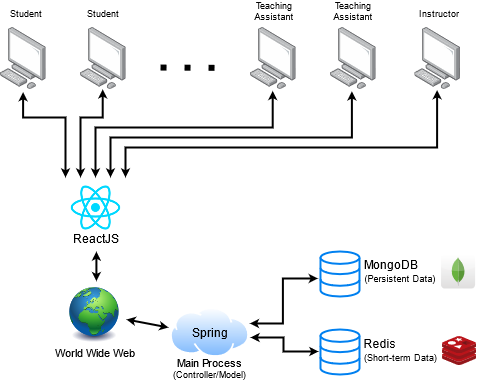
\includegraphics[width=\textwidth]{tech-diagram}
        \caption{Overlook of LabConnect's Organisation}~\label{fig:organisation-diagram}
    \end{figure}
    
    \subsection{Technologies}
    
    % TODO this subsection is almost ready on the github issue

    \pagebreak

    \section{Core Design Details}
    
    Classes are designed with the consideration of keeping them cohesive, every class only handles one concept. 


    \subsection{Class Diagram}
    
    \begin{figure}[H]
        \centering
        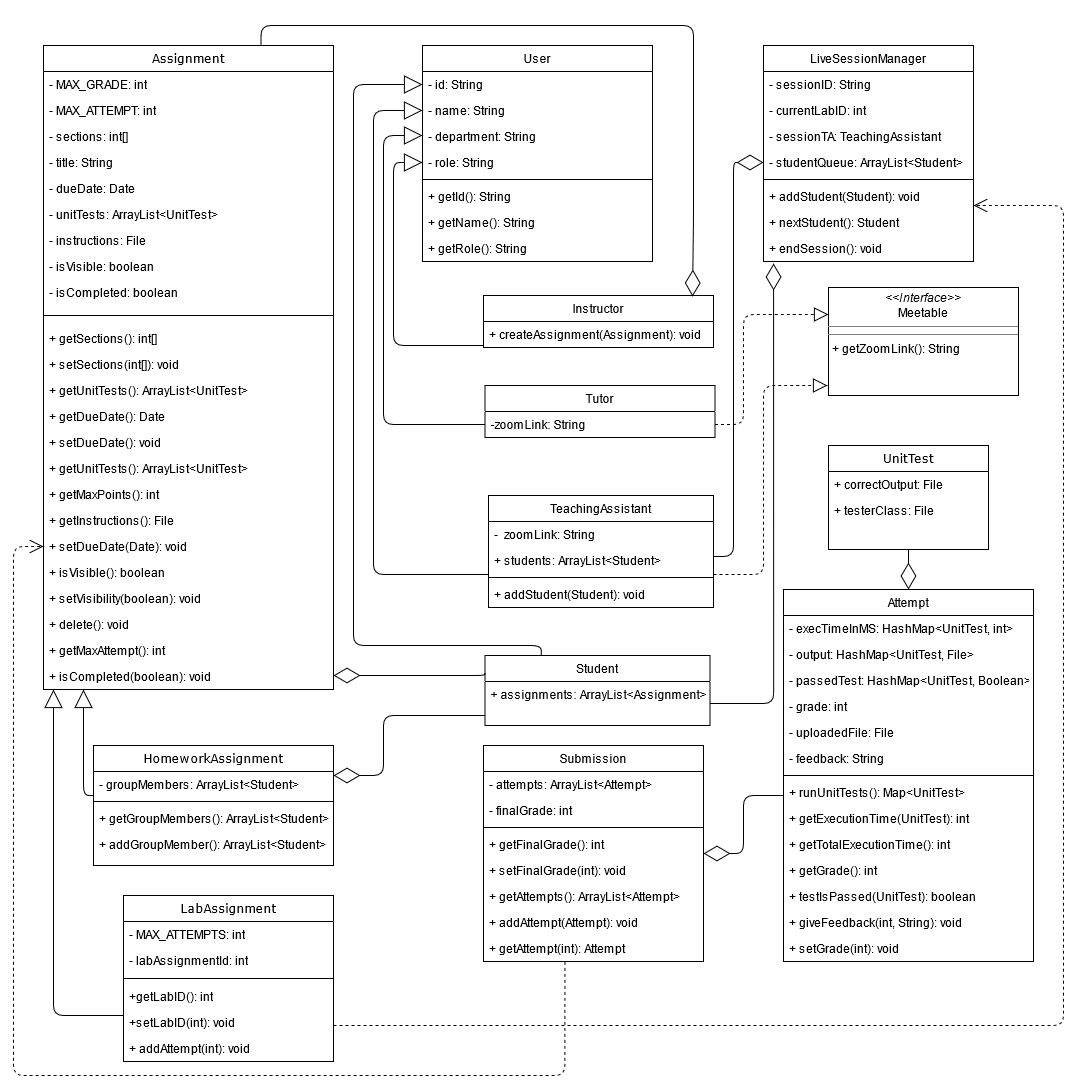
\includegraphics[width=\textwidth]{ClassUML}
        \caption{UML Class Diagram for LabConnect}~\label{fig:class-diagram}
    \end{figure}

   %\subsection{Sequence Diagram}
    
   \pagebreak
    
    \section{Task Assignment}
    
    \underline{Model Implementation Assignment:}
    \newline\newline Borga Haktan Bilen: Assignment, User, LiveSessionManager
    \newline Vedat Eren Arıcan: Assginment, Instructor, Meetable 
    \newline Berkan Şahin: Assignment, Tutor, UnitTest
    \newline Berk Çakar: Assignment, TeachingAssistant, Attempt
    \newline Alp Ertan: Assignment, Student, Submission, HomeworkAssignment, LabAssignment 
    \newline\newline For the other parts of the implementation, we agreed on sharing those parts pairwise equally 
    because of the project's size. We made this decision because one of the primary goal of our group is
    learning new concepts and gaining experiences. Thus, it will not be even for other members of the group
    who did not work on the part which involves new technologies.
    
    
        
\end{document}
